\section{Method}
This chapter gives the details of the networks and clustering algorithms that were examined. The unsupervised feature representation learning approach proposed by Guofeng Mei \textit{et. al.}\cite*{mei2022unsupervised} was adapted to be used in our scenario. The authors proposed an unsupervised learning approach, ConClu that learns both the local features and well as the global features of the point clouds. It was suitable to be used in out scenario, as it would require no point-level annotation of the dataset, which was unavailable in our case. To do so, it performed point-level clustering of the points clouds to generate semantically related regions within the point cloud and performed instance-level contrasting to make the network robust to its global appearance which I would explain in detail in the following subsections.\cite*{mei2022unsupervised}.

\vspace{5 mm}

The primary motivation behind using an unsupervised learning  methodology is that annotation of point clouds can be really challenging. To really focus on the point level features of a point cloud, one would require a high number of points in the point cloud. And labelling such high number of points in each point cloud in large real world datasets can be really expensive and severely inefficient. Unsupervised learning enables us to get high quality feature representation without the need for humans in the loop. Moreover, sporadic and non-uniform distribution of the point clouds can also add further challenges in point-level annotation of the point clouds. Thus, in the absence of such annotations, it is impossible to get supervised feature representations for computer vision tasks.

\subsection{Architecture}
\begin{figure}[t]
    \centering
    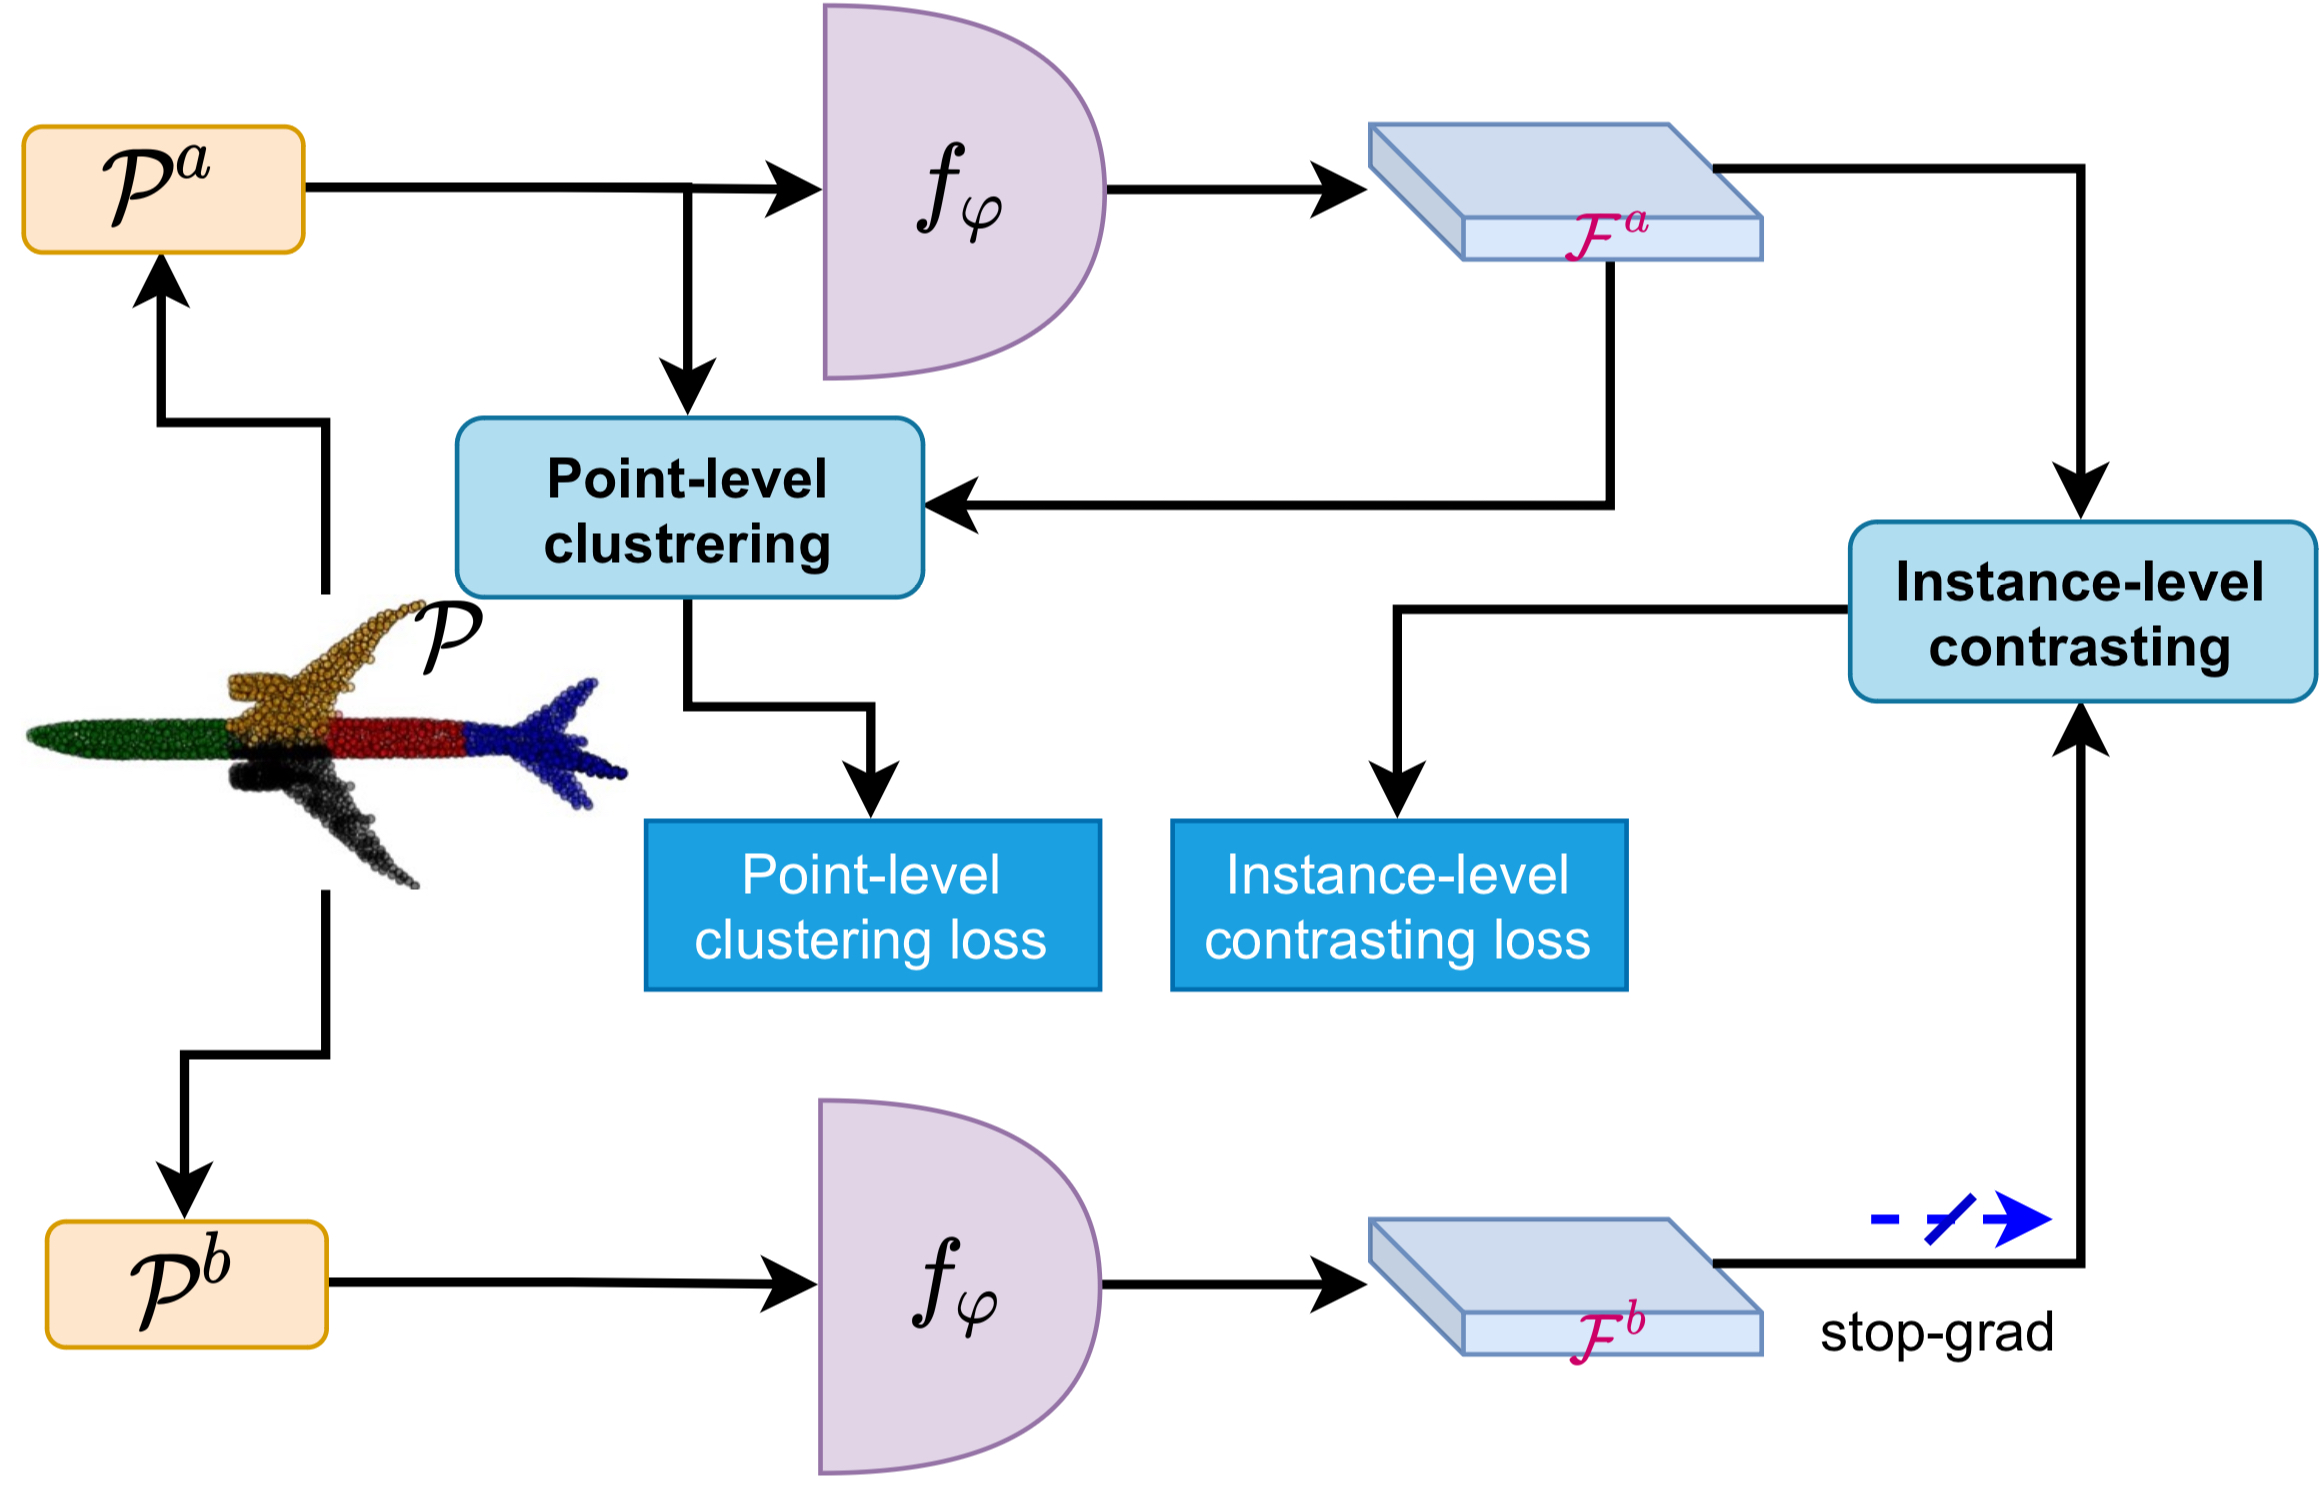
\includegraphics[width=320pt,height=200pt]{pictures/conclu_arch.jpg}
    \caption{The Conclu model pipeline including the two modules: point -level clustering and instance-level contrasting.\cite{mei2022unsupervised}}
    \label{fig:conclu_arch}
\end{figure} 
If we think about how humans perceive an object, we do not focus merely on the individual points but rather semantically related points that form a group and act as the fundamental block for the entire object as a whole. The global features focus on the entire shape of the object while the local features attains to the more detailed information in the different parts of the object. In this work, we have 3D point cloud $\mathcal{\textbf{P}} = \{\textbf{p}_i \in \mathbb{R}^3| i= 1,2,3,....,N\}$ where $N$ is the number of points in each point cloud and $\textbf{p}_i$ is each point in the point cloud representated in 3D cartesian coordinate system. The point cloud $\mathcal{\textbf{P}}$ is fed to an encoder backbone $f_{\psi}$ which generates a point-wise feature matrix $\mathcal{\textbf{F}} = \{ f_{p_i}\}_{i=1}^{N}$ where $f_{p_i}$ is the point-wise feature vector. The objective was to train a feature encoder $f_{\psi}$, PointNet in our case, having parameters $\psi$ in an unsupervised learning paradigm. The entire pipeline of the process is elaborated in Fig.\ref*{fig:conclu_arch}. As we can see, it has two parts: the point-level clustering for learning the local features and the instance-level contrasting for learning the global features. Before we go into a detailed analysis of each module, here is a brief overview of the entire process. The augmented views $\mathcal{\textbf{P}}^a$, and $\mathcal{\textbf{P}}^b$ are obtained for each point cloud $\mathcal{\textbf{P}}$ and are fed to the encoder $f_{\psi}$ such that it generates the feature matrices $\mathcal{\textbf{F}}^a$, and $\mathcal{\textbf{F}}^b$ respectively. Thus, the inputs to the point-level clustering are $\mathcal{\textbf{P}}^a$ and $\mathcal{\textbf{F}}^a$. It is to be noted here that the feature encoder $f_{\psi}$ shares the weights between the two augmented views. $f_{\psi}$ is trained in a way such that it minimises the point-level clustering and the instance-level contrasting loss together. It is also to be noted here, that the encoder receives the gradient only from the top branch. After the training is completed, both the loses are cast aside and only the encoder is needed for further tasks.

\subsection{Point-level Clustering Module}
\begin{figure}[t]
    \centering
    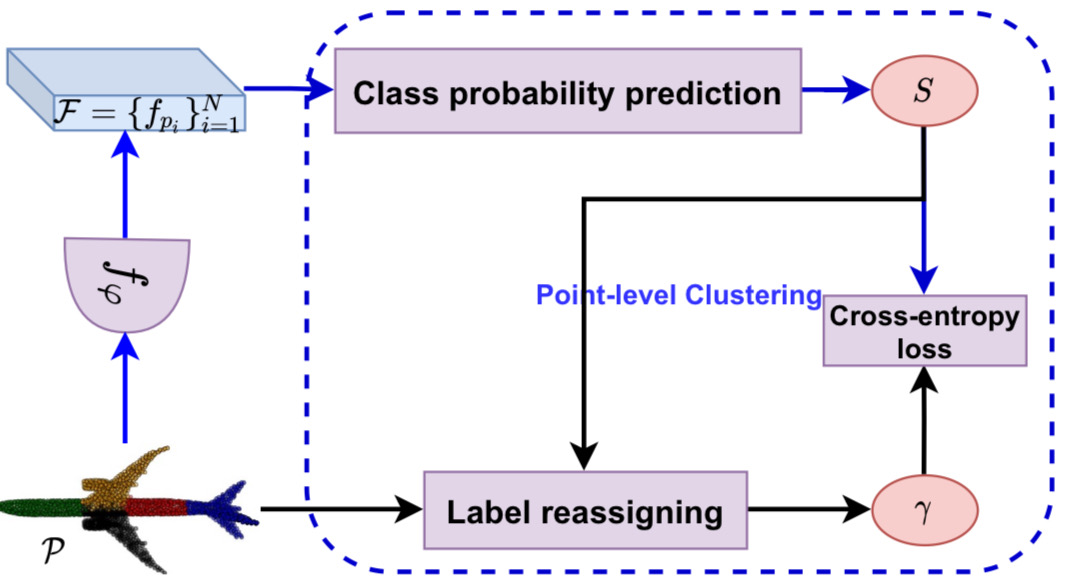
\includegraphics[width=300pt,height=180pt]{pictures/point_level.jpg}
    \caption{The architecture of the point-level clustering based unsupervised feature learning.\cite{mei2022unsupervised}}
    \label{fig:point_level}
\end{figure} 
Fig.\ref*{fig:point_level} gives a detailed visualisation of the point-level clustering module. We can see that it is made up of 2 entites, the "class probability prediction" function and the "label reassigning". The point-level clustering module is analogous to the semantic segmentation task. Each point $p_i$ of the point cloud $\mathcal{\textbf{P}}$ is assigned to one of the $J$ predetermined possible subgroups or semantic categories. Essentially, it is achieved by processing each of the point cloud $\mathcal{\textbf{P}}$ followed by a point-level class probability prediction operator that yields a matrix for class probability $\mathit{\textbf{S}} = \{ s_{ij} \in [0,1]\}_{i,j}^{N,J}$. The label reassigning operator thus takes the point cloud $\mathcal{\textbf{P}}$ and the class probability matrix $S$ and generates a pseudo-label matrix $\mathit{\mathbf{\gamma}} = \{ \gamma_{ij} \in \{0,1\}\}_{i,j}^{N,J}$. The weights for the encoder $f_{\psi}$ are learnt such that it minimizes the average cross-entropy loss between the pseudo-label $\gamma$ and the predicted class probability $\textbf{S}$. The average cross entropy loss is calculated by the formula given in Eq.\ref*{eq:avg_cross_entropy}.
\begin{equation}
    \label{eq:avg_cross_entropy}
    \mathit{\epsilon}(\gamma,\textbf{S})= \mathit{ - \frac{1}{N}} \langle \gamma,\log \textbf{S} \rangle = \mathit{ - \frac{1}{N}} \sum_{i=1}^{N} \sum_{j=1}^{J} \gamma_{ij} \log s_{ij}
\end{equation}
But to train a network with a cross-entropy loss, the ground truth labels of the points in the point cloud are required. Since that is not available, one needs to assign the label $\gamma$ automatically, which is explained in details in the following passage. 

\subsubsection{Class Probability prediction}
As mentioned in the last passage, the output of the encoder $f_{\psi}$ is fed as input to a classification head $\phi_\alpha$ and it generates a logit score for each of the feature vector as shown in Fig.\ref*{fig:class_prob}. The vector for the logit score if given by $\textbf{g}_i = (g_{i1}, g_{i2},....., g_{iJ}), where \textbf{g}_i = \gamma_\alpha(f_{p_i})$. The classification head has 2 fully connected layers where each layer is a linear layer followed by a batch normalization. The leakyreLU activation function is used in all the layers except the last layer. As the output of the last layer we get N vectors for each of the N points in the point cloud where each of the output vector has $J$ dimensions, the number of predetermined subcategories each point cloud is to be segmented into. Thus each entry of the feature vector is the probability of that point belonging to $j-th$ category. Thus, the logit score matrix $\textbf{G} = \{ g_{ij}\}_{i,j}^{N,J}$ has the dimension $N \times J$. The prediction that the point $p_i$ belongs to the category $j$ is computed by teh application of a row-wise softmax operation on $\textbf{G}$ given by Eq.\ref*{eq:softmax}
\begin{equation}
    \label{eq:softmax}
    \mathit{s_{ij}}= \mathit{\frac{exp(g_{ij})}{\sum_{l=1}^{J}exp(g_{ij})}} 
\end{equation}

\begin{figure}
    \centering
    \begin{minipage}[t]{.45\textwidth}
      \centering
      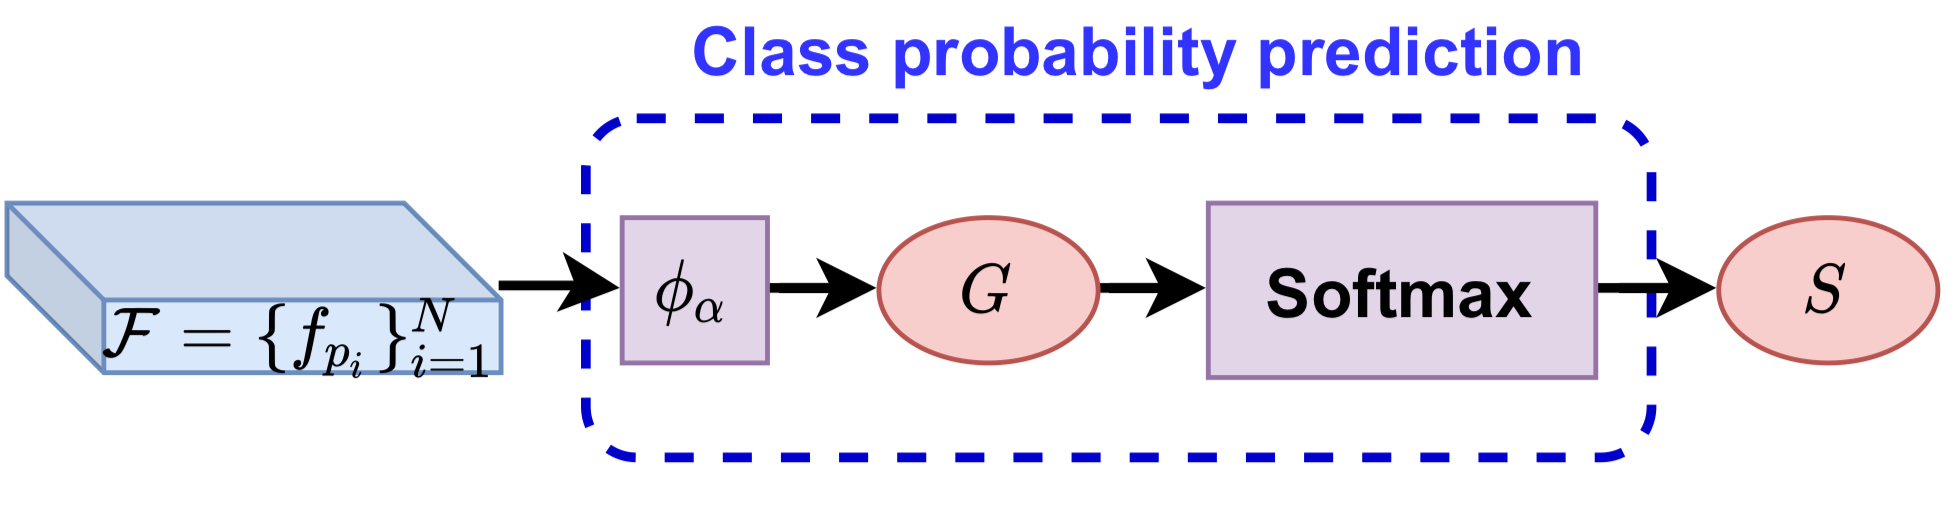
\includegraphics[width=200pt,height=100pt]{pictures/class_prob.jpg}
      \captionof{figure}{Architecture of class probability prediction.\cite{mei2022unsupervised}}
      \label{fig:class_prob}
    \end{minipage}%
    \hspace{1cm}
    \begin{minipage}[t]{.45\textwidth}
      \centering
      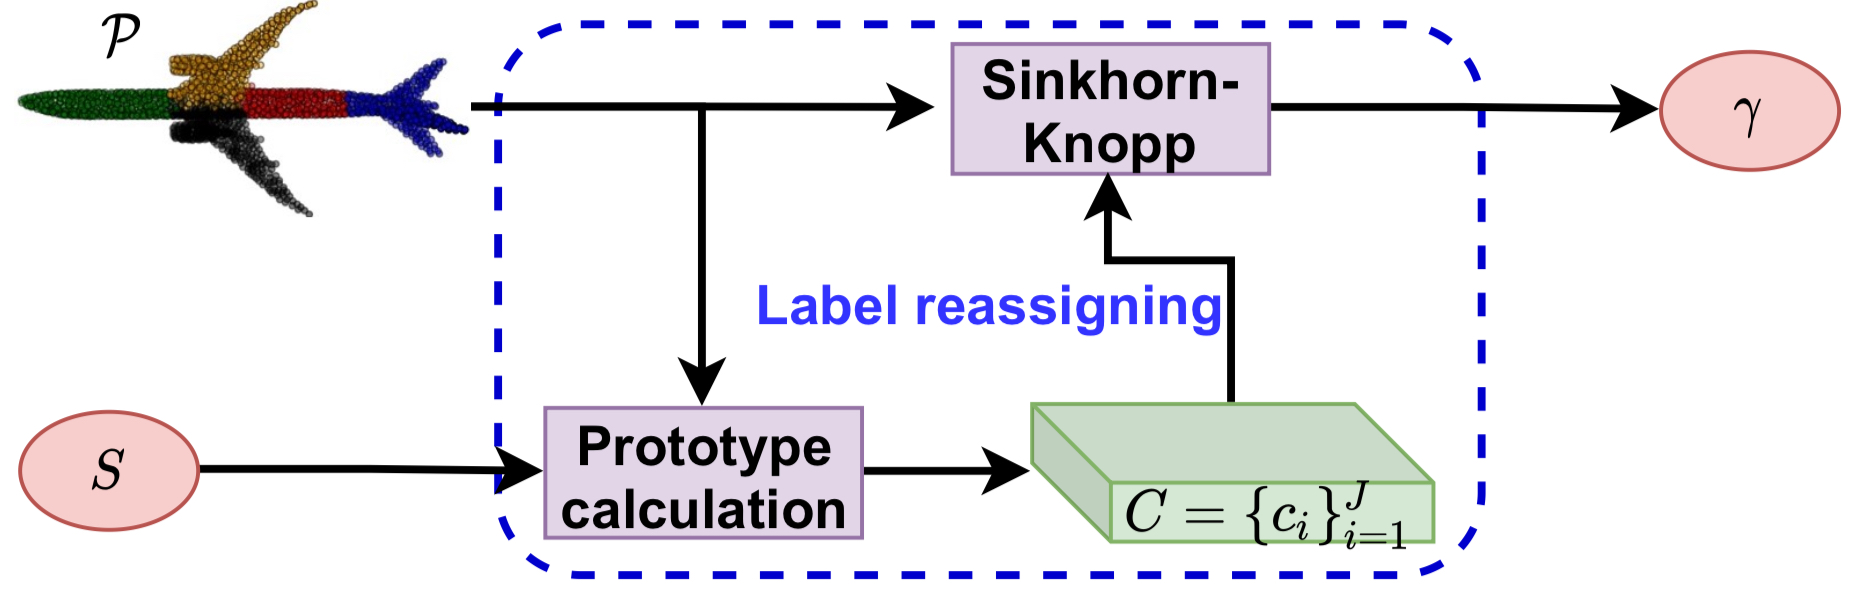
\includegraphics[width=200pt,height=100pt]{pictures/label_reassign.jpg}
      \captionof{figure}{Architecture of label reassigning \cite{mei2022unsupervised}}
      \label{fig:label_reassign}
    \end{minipage}
\end{figure}
\todo{Continue from label reassigning}

\subsection{Suitable Algorithm and Adjustments}
\subsection{Whatever new Concept we propose}
\subsection{Architecture}
\subsection{Source and Target Objects}
\subsection{Data Generation}
\subsection{Important Aspects}